\section{Incompressible Navier-Stokes Solver}

3.4/UserGuide/Tutorial/IncNavierStokesSolver
3.4/UserGuide/Tutorial/IncNavierStokesSolver/Stability
3.4/UserGuide/Examples/IncNavierStokesSolver/Adjoint
3.4/UserGuide/Examples/IncNavierStokesSolver/Aorta
3.4/UserGuide/Examples/IncNavierStokesSolver/Biglobal
3.4/UserGuide/Examples/IncNavierStokesSolver/Direct
3.4/UserGuide/Examples/IncNavierStokesSolver/KovasznayFlow2D
3.4/UserGuide/Examples/IncNavierStokesSolver/LaminarChannelFlow2D
3.4/UserGuide/Examples/IncNavierStokesSolver/LaminarChannelFlow2DLinNS
3.4/UserGuide/Examples/IncNavierStokesSolver/LaminarChannelFlow3D

3.4/UserGuide/Examples/IncNavierStokesSolver/LaminarChannelFlow3DH1D

\subsection{Laminar Channel Flow Quasi-3D}

In this example we reuse the 2D mesh used before for the \hyperref{2D Laminar Channel Flow} example, and we add mathematically the third dimension assuming an expansion along z with a Fourier series. The example is an application of the IncNavierStokesSolver using the Velocity Correction Scheme algorithm.

\subsubsection{Background}

The governing equation is the unsteady incompressible Navier-Stokes equation:
\begin{equation}
\begin{cases}
\frac{\partial \textbf{u}}{\partial t} + \textbf{u} \cdot \nabla \textbf{u} = - \nabla p + \nu \nabla^2 \textbf{u} + f \\
\nabla \cdot \textbf{u} = 0
\end{cases}
\end{equation}

The Reynolds number under consideration is 1.

\subsubsection{Geometry}

The geometry under consideration is a 2D square channel with unit length and height (\textit{i.e.} $D=1$). The channel is modelled using 4 quadrilateral elements. The geometry as well as the mesh is identical to that used in the 2D Laminar Channel Flow example.

\subsubsection{Input parameters}

\paragraph{Expansion:~} In this example we will use a quadratic polynomial expansion (\textit{i.e.} $P=3$).
\begin{lstlisting}[style=XMLStyle]
<EXPANSIONS>
  <E COMPOSITE="C[0]" NUMMODES="3" FIELDS="u,v,w,p" TYPE="MODIFIED" />
</EXPANSIONS>
\end{lstlisting}

\paragraph{Solver information:~}  The flag 
\begin{lstlisting}[style=XMLStyle] 
<I PROPERTY="HOMOGENEOUS" VALUE="1D"/> 
\end{lstlisting} 
is informing the code that, even if the mesh is 2D, the problem is 3D and the third direction needs to be added with a Fourier series. An extra flag could be added to activate the FFT routines inside the code 
\begin{lstlisting}[style=XMLStyle]
<I PROPERTY="USEFFT" VALUE="FFTW"/>
\end{lstlisting} 

In this case Nektar++ uses the FFTW library to move the degrees of freedom from wave to real space. HomModesZ and LZ set the number of Fourier modes and the length of the third direction respectively.
\begin{lstlisting}[style=XMLStyle]
  <SOLVERINFO>
    <I PROPERTY="EQTYPE" VALUE="UnsteadyNavierStokes"/>
    <I PROPERTY="SolverType"  VALUE="VelocityCorrectionScheme"/>
    <I PROPERTY="EvolutionOperator" VALUE="Nonlinear" />
    <I PROPERTY="Projection" VALUE="Galerkin"/>
    <I PROPERTY="TimeIntegrationMethod" VALUE="IMEXOrder3"/>
    <I PROPERTY="HOMOGENEOUS" VALUE="1D"/>
  </SOLVERINFO>
\end{lstlisting}

\paragraph{Parameters:~} Setting the mean inlet velocity to 1, allows us to define the kinematic viscosity as $\nu = \frac{UD}{Re}=1$.
\begin{lstlisting}[style=XMLStyle]
  <PARAMETERS>
    <P> TimeStep      = 0.001    </P>
    <P> NumSteps      = 1000     </P>
    <P> IO_CheckSteps = 1000     </P>
    <P> IO_InfoSteps  = 1000     </P>
    <P> Kinvis        = 1        </P>
    <P> HomModesZ     = 20       </P>
    <P> LZ            = 1.0      </P>
  </PARAMETERS>
\end{lstlisting}

\paragraph{Boundary conditions:~} Boundary conditions have been defined on the walls and at the inflow (regions 0 and 1) as Dirichlet for the velocity field and as high-order for the pressure. At the outflow the velocity is left free using Neumann boundary conditions and the pressure is set to zero using Dirichlet.
\begin{lstlisting}[style=XMLStyle]
  <BOUNDARYCONDITIONS>
    <REGION REF="0">
      <D VAR="u" VALUE="0" />
      <D VAR="v" VALUE="0" />
      <D VAR="w" VALUE="0" />
      <N VAR="p" USERDEFINEDTYPE="H" VALUE="0" />
    </REGION>
    <REGION REF="1">
      <D VAR="u" VALUE="y*(1-y)" />
      <D VAR="v" VALUE="0" />
      <D VAR="w" VALUE="0" />
      <N VAR="p" USERDEFINEDTYPE="H" VALUE="0" />
    </REGION>
    <REGION REF="2">
      <N VAR="u" VALUE="0" />
      <N VAR="v" VALUE="0" />
      <N VAR="w" VALUE="0" />
      <D VAR="p" VALUE="0" />
    </REGION>
  </BOUNDARYCONDITIONS>
\end{lstlisting}

\paragraph{Functions:~} Homogeneous initial conditions are imposed and an analytical formulation of the exact solution is provided.
\begin{lstlisting}[style=XMLStyle]
  <FUNCTION NAME="InitialConditions">
     <E VAR="u" VALUE="0" />
     <E VAR="v" VALUE="0" />
     <E VAR="w" VALUE="0" />
     <E VAR="p" VALUE="0" />
  </FUNCTION>

  <FUNCTION NAME="ExactSolution">
     <E VAR="u" VALUE="y*(1-y)" />
     <E VAR="v" VALUE="0" />
     <E VAR="w" VALUE="0" />
     <E VAR="p" VALUE="-2*Kinvis*(x-1)" />
  </FUNCTION>
\end{lstlisting}

\subsubsection{Usage}
./IncNaverStokesSolver session.xml

\subsubsection{Result}

\begin{figure}
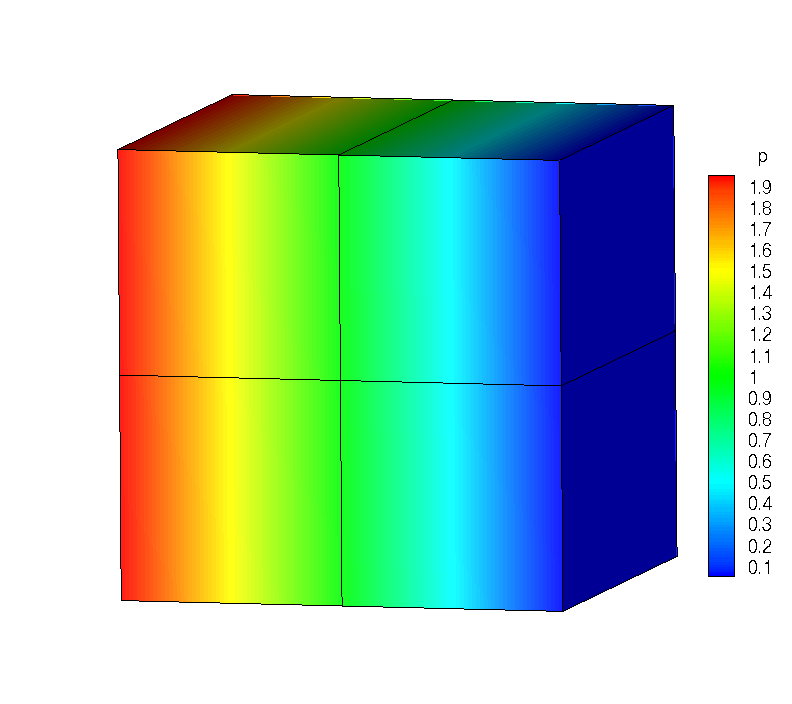
\includegraphics[width=7cm]{Figures/CF3DCVP3PR.png}
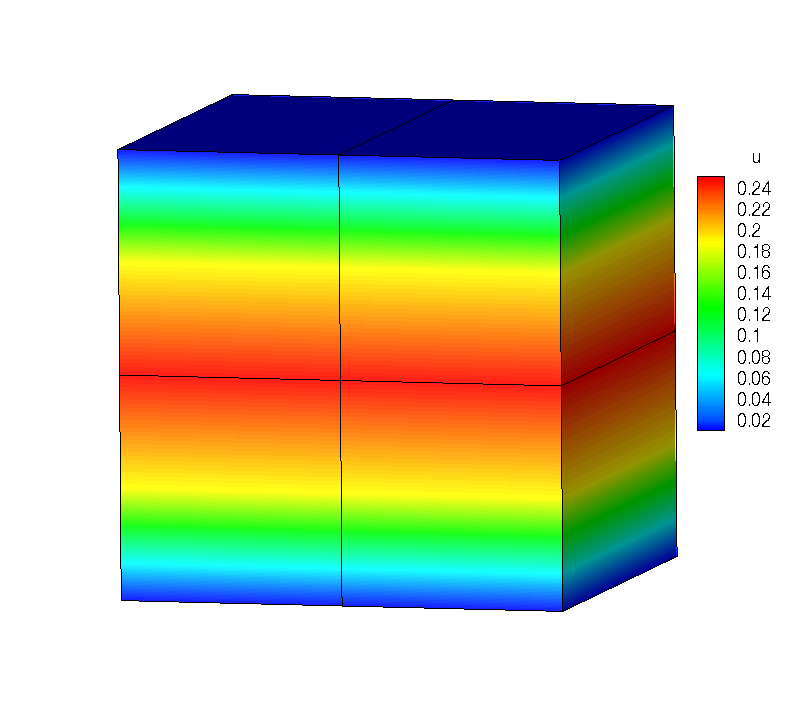
\includegraphics[width=7cm]{Figures/CF3DCVP3.png}
\end{figure}









3.4/UserGuide/Examples/IncNavierStokesSolver/SteadyOseenFlow2D
3.4/UserGuide/Examples/IncNavierStokesSolver/Transient
3.4/UserGuide/Examples/IncNavierStokesSolver/TurbulentChannelFlow
3.4/UserGuide/Examples/IncNavierStokesSolver/TurbulentPipeFlow

